\documentclass{article}
\usepackage{tikz}
\usepackage[margin=2cm]{geometry}
\begin{document}

\section*{Juring, Tembereng, dan Apotema Lingkaran}

\subsection*{Juring: potongan yang titiknya di pusat}
Lingkaran berjari-jari 3 cm, sudut pusat $60^\circ$. Luas juring $= \frac{60}{360} \times \pi \times 3^2 = 1{,}5\pi \approx 4{,}71$ cm$^2$.
\begin{center}
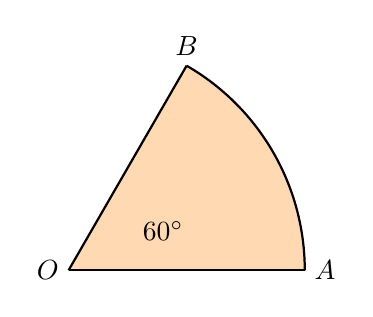
\begin{tikzpicture}[scale=1]
  \coordinate (O) at (0,0);
  \coordinate (A) at (3,0);
  \coordinate (B) at (1.5,2.6);
  \fill[orange!30] (O) -- (A) arc (0:60:3) -- cycle;
  \draw[thick] (O) -- (A);
  \draw[thick] (O) -- (B);
  \draw[thick] (A) arc (0:60:3);
  \node[left] at (O) {$O$};
  \node[right] at (A) {$A$};
  \node[above] at (B) {$B$};
  \node at (1.2,0.5) {$60^\circ$};
\end{tikzpicture}
\end{center}

\subsection*{Tembereng: daerah antara tali busur dan busur}
Lingkaran berjari-jari 3 cm, sudut pusat $120^\circ$. Luas tembereng $\approx 3\pi - 3{,}90 \approx 5{,}52$ cm$^2$.
\begin{center}
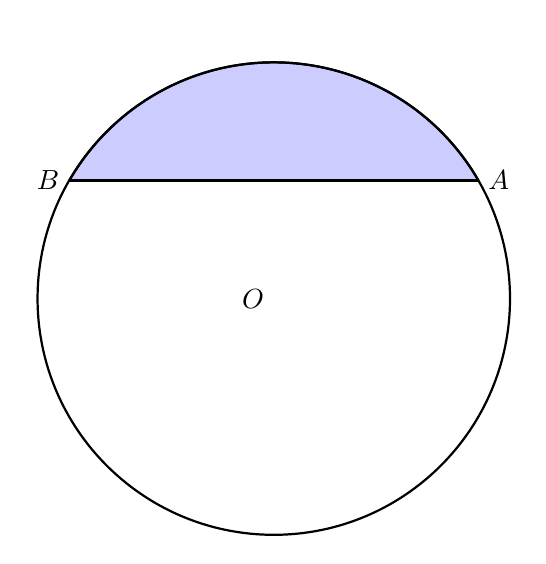
\begin{tikzpicture}[scale=1]
  \coordinate (O) at (0,0);
  \coordinate (A) at (2.6,1.5);
  \coordinate (B) at (-2.6,1.5);
  \fill[blue!20] (A) arc (30:150:3) -- cycle;
  \draw[thick] (O) circle (3);
  \draw[thick] (A) -- (B);
  \draw[thick] (A) arc (30:150:3);
  \node[left] at (O) {$O$};
  \node[right] at (A) {$A$};
  \node[left] at (B) {$B$};
\end{tikzpicture}
\end{center}

\subsection*{Apotema: garis tegak lurus dari pusat ke tali busur}
Lingkaran berjari-jari 5 cm, tali busur 8 cm, apotema $= \sqrt{5^2 - 4^2} = 3$ cm.
\begin{center}
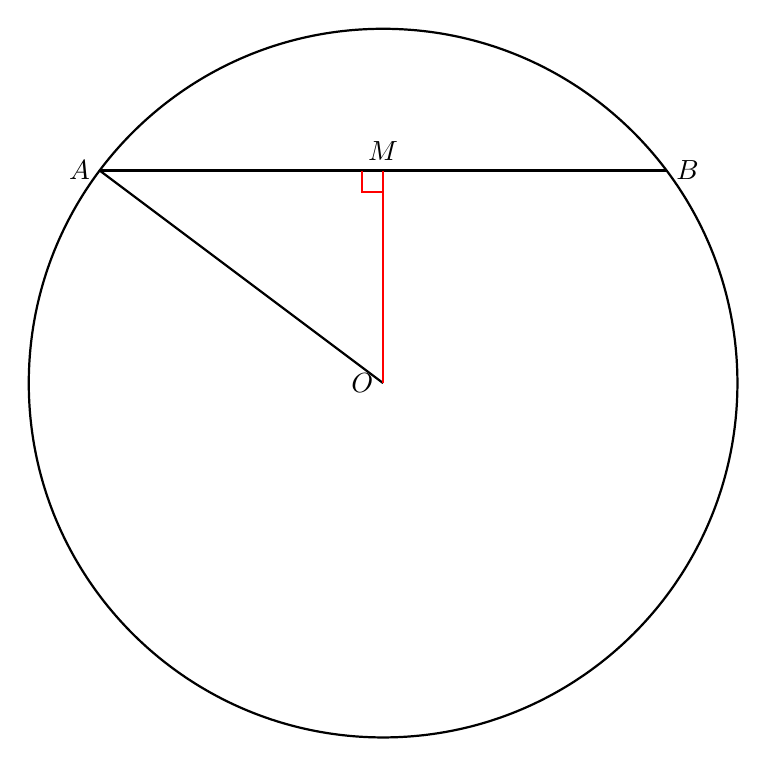
\begin{tikzpicture}[scale=0.9]
  \coordinate (O) at (0,0);
  \coordinate (A) at (-4,3);
  \coordinate (B) at (4,3);
  \coordinate (M) at (0,3);
  \draw[thick] (O) circle (5);
  \draw[thick] (O) -- (A);
  \draw[thick] (A) -- (B);
  \draw[red, thick] (O) -- (M);
  \draw[red, thick] (M) ++(-0.3,0) -- ++(0,-0.3) -- ++(0.3,0);
  \node[left] at (O) {$O$};
  \node[left] at (A) {$A$};
  \node[right] at (B) {$B$};
  \node[above] at (M) {$M$};
\end{tikzpicture}
\end{center}

\end{document}
